\subsection[web]{Web tools}

\begin{frame}
  \frametitle{Godbolt / Compiler Explorer }
  \begin{block}{Concept}
    An online generic compiler with immediate feedback.
    Allows:
    \begin{itemize}
    \item compiling online any code against any version of any compiler
    \item inspecting the assembly generated
    \item use of external libraries (over 50 available !)
    \item running the code produced
    \item using tools, e.g. ldd, include-what-you-use, ...
    \item sharing small pieces of code via permanent short links
    \end{itemize}
  \end{block}
  \begin{exampleblock}{Typical usage}
    \begin{itemize}
    \item check small pieces of code on different compilers
    \item check some new \cpp functionality and its support
    \item optimize small pieces of code
    \item NOT relevant for large codes
    \end{itemize}
  \end{exampleblock}
\end{frame}

\begin{frame}
  \frametitle{Godbolt by example}
  \begin{block}{Check effect of optimization flags}
    \url{https://godbolt.org/z/Pb8WsWjEx}
    \begin{itemize}
    \item Check generated code with -O0, -O1, -O2, -O3
    \item See how it gets shorter and simpler
    \end{itemize}
  \end{block}
  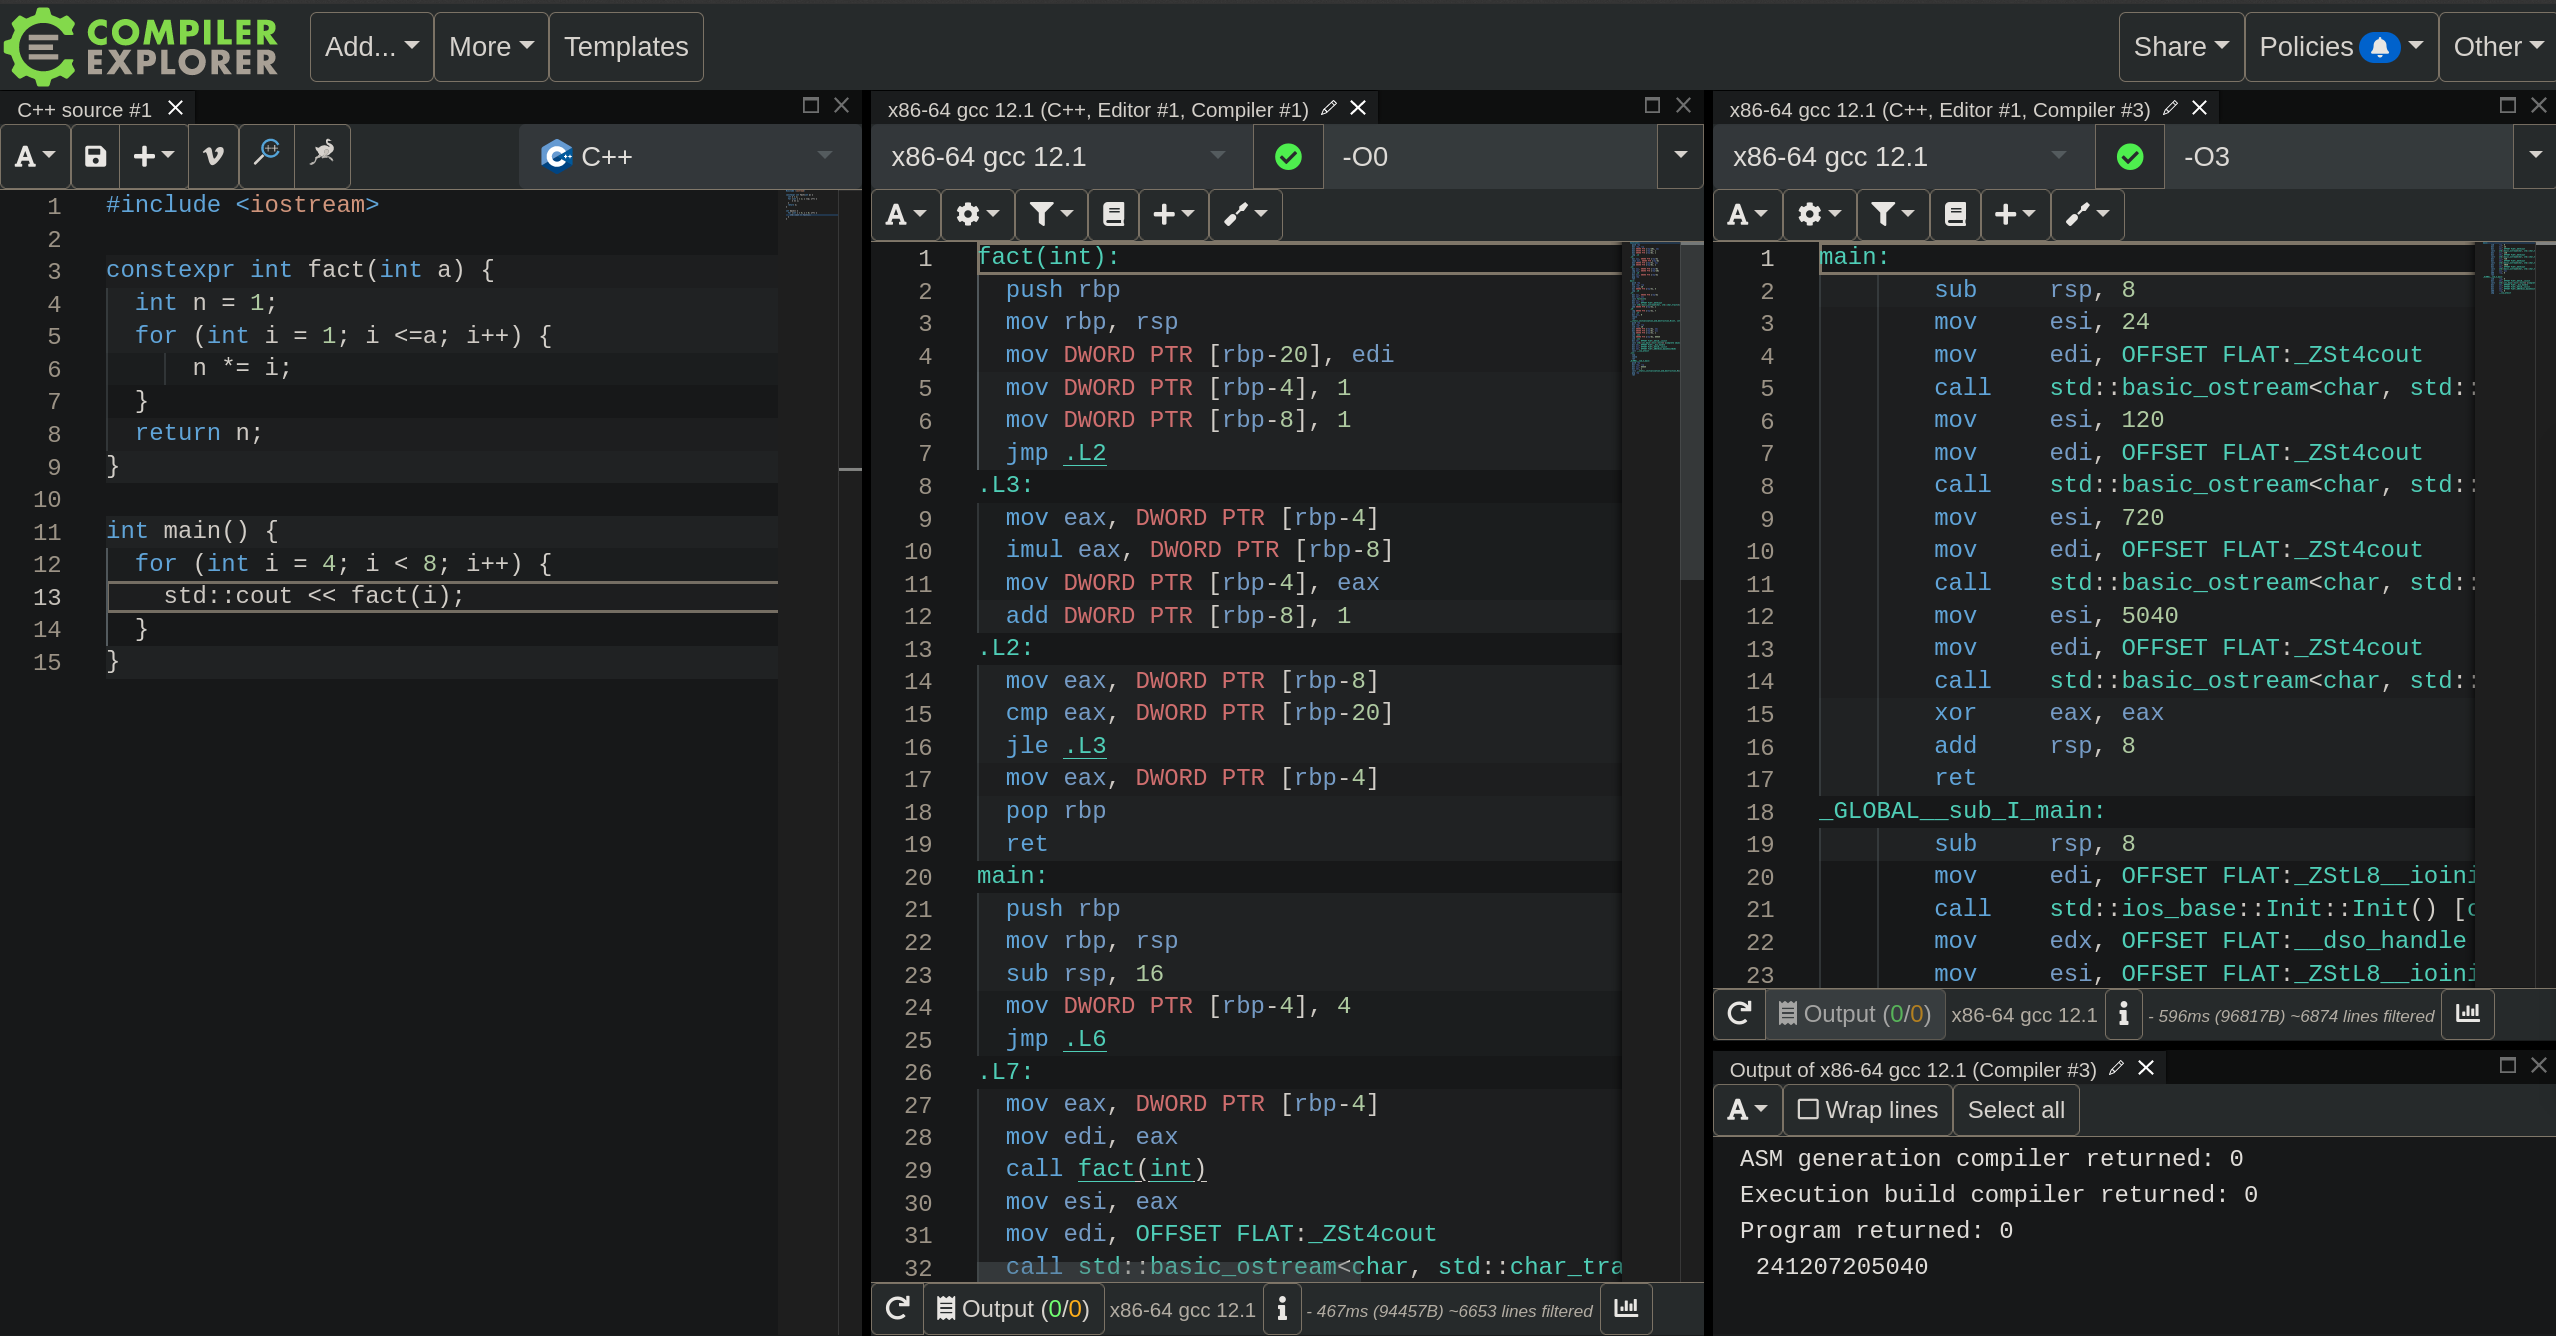
\includegraphics[width=\textwidth]{tools/godbolt.png}
\end{frame}

\begin{frame}
  \frametitle{cppinsights}
  \begin{block}{Concept}
    Reveals the actual code behind \cpp syntactic sugar
    \begin{itemize}
    \item lambdas
    \item range-based loops
    \item templates
    \item initializations
    \item auto
    \item ...
    \end{itemize}
  \end{block}
  \begin{exampleblock}{Typical usage}
    \begin{itemize}
    \item understand how things work behind the \cpp syntax
    \item debug some non working pieces of code
    \end{itemize}
  \end{exampleblock}
\end{frame}

\begin{frame}
  \frametitle{cppinsights by example}
  \begin{block}{Check how range-based loop work}
    \url{https://cppinsights.io/s/b886aa76}
    \begin{itemize}
    \item See how they map to regular iterators
    \item And how operators are converted to function calls
    \end{itemize}
  \end{block}
  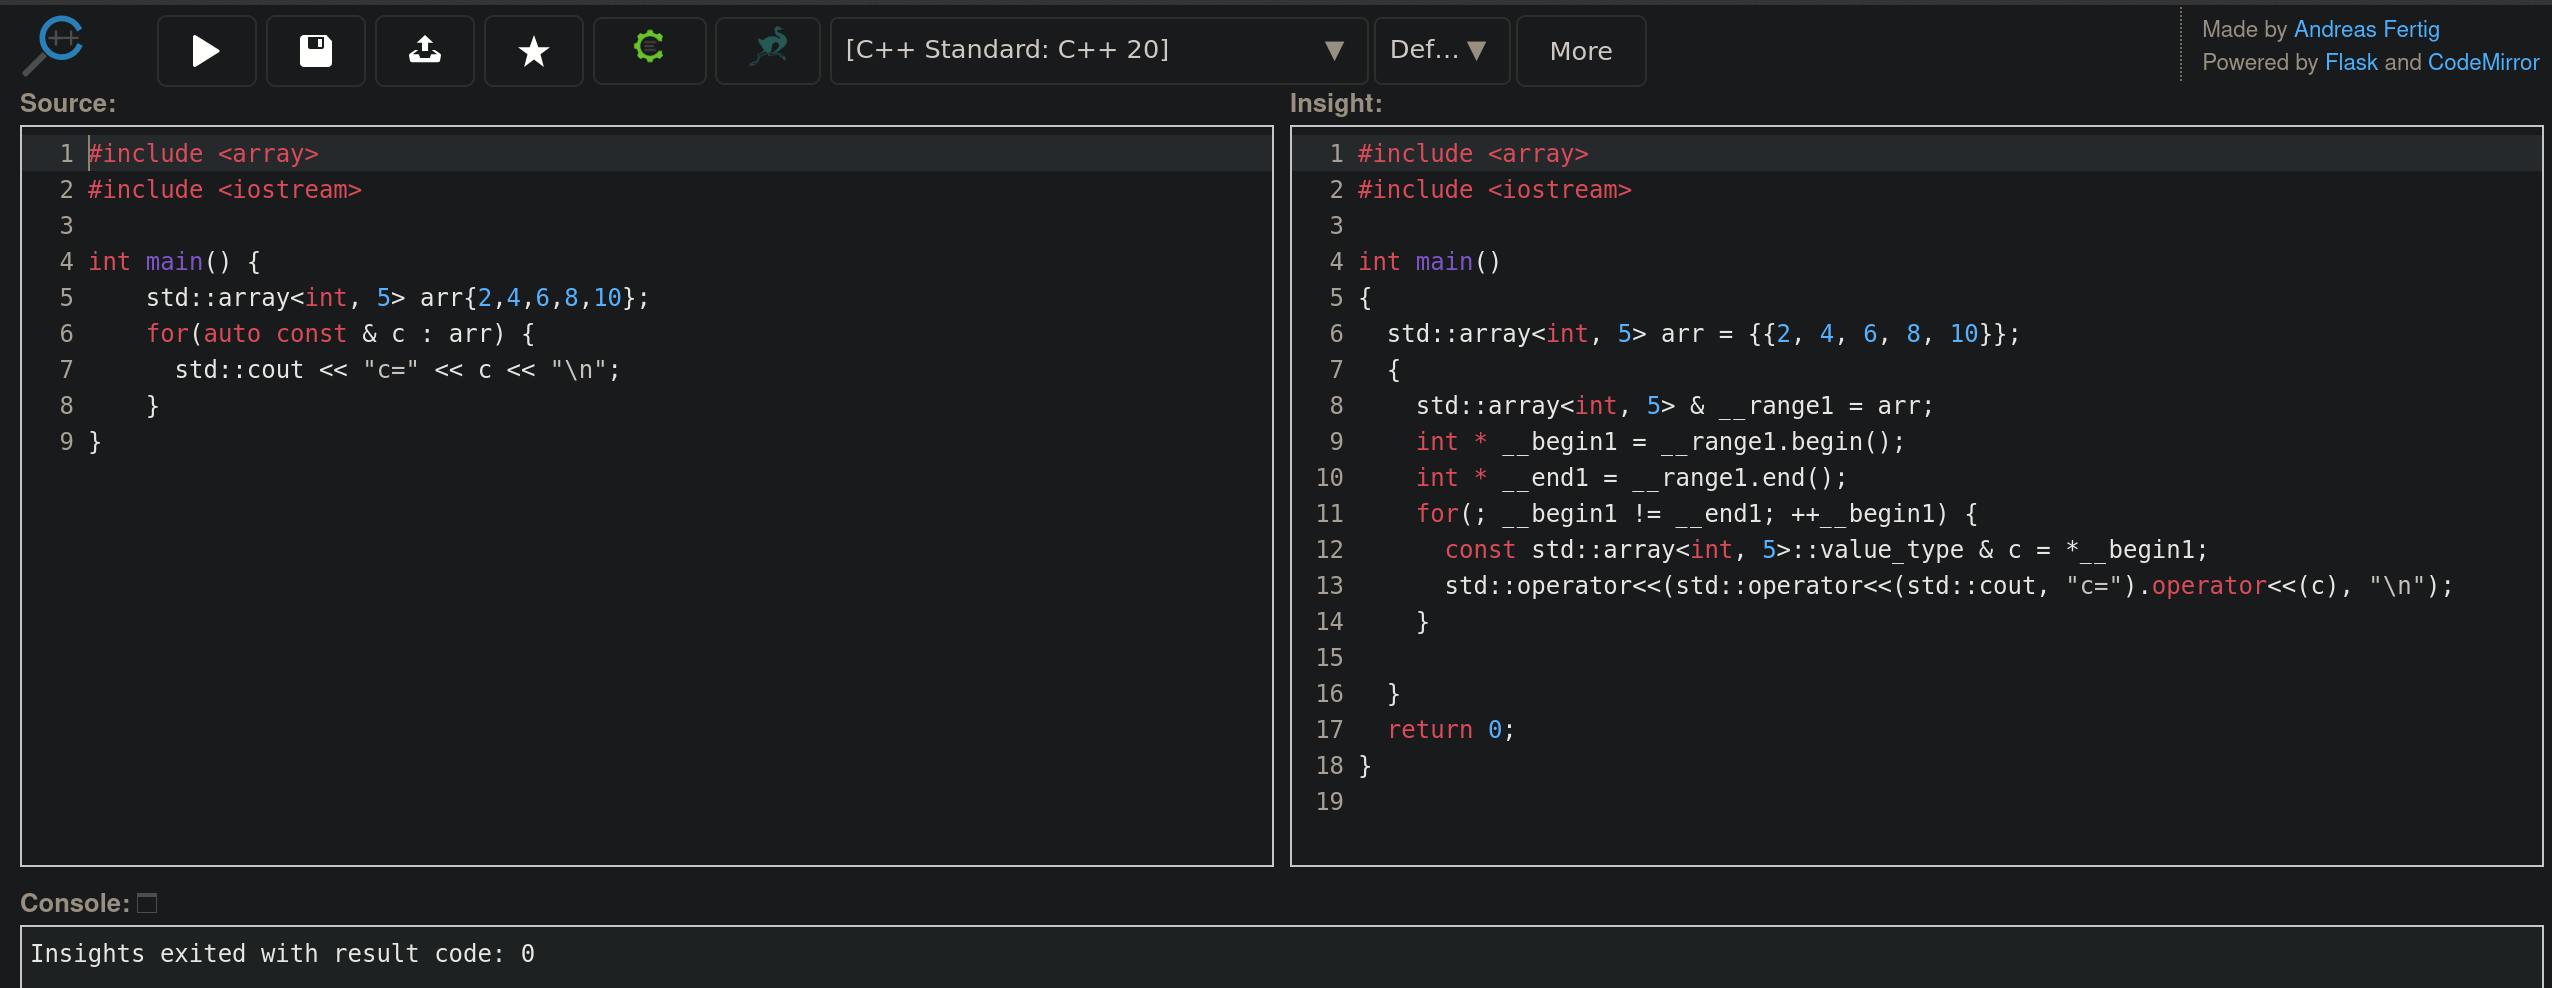
\includegraphics[width=\textwidth]{tools/cppinsights.png}
\end{frame}
